\documentclass[10pt]{article}
\usepackage[T1]{fontenc}
\usepackage[utf8]{inputenc}
\usepackage[brazilian]{babel}
\usepackage{hyphenat}
\usepackage{amsmath,amssymb,calrsfs,physics}
\usepackage[a4paper, margin=2cm]{geometry}
\usepackage{graphicx}
\graphicspath{ {./images/} }
\usepackage{textcomp}
\usepackage[export]{adjustbox}
\usepackage{multirow}
\usepackage{subcaption}
\usepackage{wrapfig}
\usepackage[colorlinks=true,linkcolor=blue]{hyperref}%
\usepackage{microtype} 			% para melhorias de justificação
\usepackage[ruled,vlined]{algorithm2e}
\usepackage{csquotes}
\usepackage{float}
\usepackage{tabularx}
\usepackage[backend=biber, style=ieee, sorting=ynt]{biblatex}
\addbibresource{refs.bib}

\begin{document}
\title{
    Exercício Latex I \\
    \large PFC1}

\begin{figure}[t]
    \centering
    
\includegraphics[scale=0.7]{images/brasao_ufmg.png}
\end{figure}

\author{Rodrigo Pimentel Faria - 2017050126}
\date{\today}
\maketitle

\section{Resumo}

Um dos artigos utilizados na pesquisa para o trabalho proposto é a dissertação \emph{An Embedded Real-Time Object Detection and Measurement of its Size} \cite{othman}. O tema principal dessa referência é o uso da biblioteca OpenCV para tirar medidas e realizar dimensionamentos de objetos em tempo real, diretamente de \emph{streams} de vídeo. A estratégia utilizada é dividida em quatro etapas que são aplicadas a cada quadro capturado, sendo elas: identificação do objeto a ser medido utilizando o algoritmo \emph{canny edge detection}, utilização de operadores morfológicos como dilatação e erosão, encontrar e selecionar os contornos e medir as dimensões do objeto.\\
Essa abordagem é extremamente relevante à aplicação desse projeto final de curso, visto que para determinar se uma célula é NG, as distâncias entre o material fotossensível e as bordas dos retângulos feitos de material condutivo, são o que determinam o alinhamento das camadas dos rolos de célula fotossensível.

\begin{figure}[H]
    \centering
    \begin{subfigure}[b]{0.49\textwidth}
        \centering
        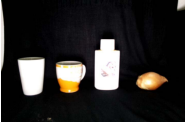
\includegraphics[scale=1.55]{images/input_image.png}
        \caption{Foto sem tratamento}
        \label{fig:celula_raw}
    \end{subfigure}
    \hfill
    \begin{subfigure}[b]{0.49\textwidth}
        \centering
        %% substituir pela imagem correta depois
        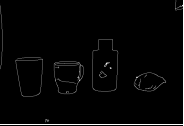
\includegraphics[scale=1.52]{images/output_image.png}
        \caption{Após algoritmo de detecção de bordas}
        \label{fig:detec_quinas}
    \end{subfigure}
    \caption{Fotos antes e depois do algoritmo de detecção de bordas}
    \label{fig:celulas}
\end{figure}

\section{Resultados}

Todas as operações de processamento de imagens realizadas na pesquisa utilizaram os módulos de \cite{opencv}. Utilizando a rotina para detecção de bordas, mesmo com a configuração da captura da foto não sendo ideal, a aplicação de operações morfológicas \ref{eq:dilation}\ref{eq:erosion} na imagem toda, é possível atingir níveis de acurácia elevados, como indicado na tabela abaixo.

\begin{equation}
    dst(x,y)=max_{(x',y'):element(x',y')!=0}src(x+x',y+y')
    \label{eq:dilation}
\end{equation}

\begin{equation}
    dst(x,y)=min_{(x',y'):element(x',y')!=0}src(x+x',y+y')
    \label{eq:erosion}
\end{equation}
\\

As operações morfológicas expressas acima \cite{morpho}, foram aplicadas de maneiras alternadas: o primeiro procedimento foi feito aplicando-se primeiramente o algoritmo da erosão, seguido da dilatação; o segundo se deu na ordem inversa, com a dilatação seguida da erosão. Com esse método, foi possível obter o resultado da imagem \ref{fig:detec_quinas}.

\begin{tabularx}{0.8\textwidth} { 
  | >{\centering\arraybackslash}X 
  | >{\centering\arraybackslash}X | }
 \hline
 \textbf{Name of objects} & \textbf{Accuracy} \\
 \hline
 white glass & 95,45 \\
 \hline
 orange cup & 97,56 \\
 \hline
 bottle & 98,23 \\
 \hline 
 potatoes & 96,82
\hline
\end{tabularx}

\printbibliography
\end{document}
